\subsubsection{Suite}\label{Testing:About:Suite}
	In this section we will talk about the testing suite and how it works and what is does.
	
	Since we chose to do most of our testing on NS3 using the MobiEmu\footnote{A framework for emulating mobile ad-hoc networks with Linux containers and ns-3. \url{https://code.google.com/p/mobiemu/}} framework most of our tests are fully automated. As we have not manage to integrate everything into the testing framework some variables are still static, but these will be highlighted where applicable.

	\begin{shaded}
	Please refer to appendix \ref{MobiEmu Setup Guide} for instruction on how to set up the testing framework. And for a description of the different variables in the test.
	\end{shaded}
	
	As we alluded to in section \ref{System testing} we had quite high hopes for how we were going to test the whole system. Unfortunately for us that did not pan out the way we wanted it to. We had some major problems regarding NS3 and how it connects its nodes to the Tap-Bridges created. This led us to having to rethink our whole test setup. We decided, after talking to the customer, that we would change the test and create a simpler network layout which would work with NS3. In figure: \ref{fig:NS3network} you can see this new altered network layout. What this means for the project is that we can not test all the functionality that we wanted to, but we are still quietly confident that we can draw some conclusion about the results. In appendix \ref{NS3 Problems} we have outlined the problems we faced and a possible solution that we did not have time to implement.
	
	\begin{figure}[H]
        \centering
        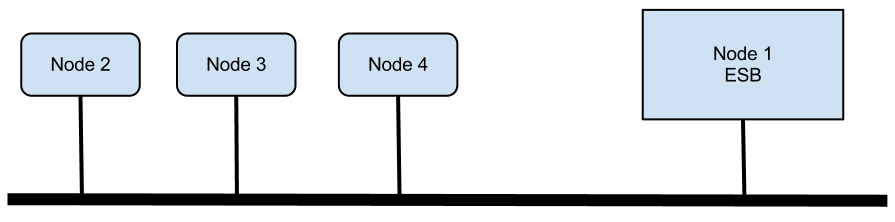
\includegraphics[width=\textwidth, scale=0.3]{NS3network}
        \caption{The layout of our network during testing}
        In this figure we have illustrated the layout of the network during NS3 testing.
        \label{fig:NS3network}
    \end{figure}
    
    This new layout does limit the scope of the test and also what we can approve of functionality, but still we think we have a strong end product with results that will absolutely be relevant for the customer.
    
    The MobiEmu testing framework operates by creating LXC and connecting these to tap bridges created by NS3. This then emulates any network possible to create in NS3. From the point of view of programs running inside the LXC, they are full Linux machines connected to a real network. This means that any program able to run on Linux should run properly inside the LXC and any messages they send out is sent through NS3. This means that we have full control over how our network behaves and we can emulate quite a lot of scenarios.
    
    When MobiEmu start up it creates a number of LXCs, it then starts up NS3 outside of any LXC and connects each of the LXCs to a corresponding tap bridge in NS3. Inside each of the LXCs it then starts the experiment and waits for the whole thing to finish before it completes nicely. Before each run MobiEmu stores all files and folders in the whole folder in order to easily recreate an experiment. When the experiment is done the result files are moved into the result folder. \\
    
    Our tests then are set up as follows. We have three clients, two clients with low priority and one client with high priority. They send messages to the ESB which is connected to the same LAN as all the clients. The specific test client we use is describe in the following section. In the section \ref{Testing:Cases} we have a detailed description of the reason behind each case. We test with several different bandwidths in order to test our setup and see how it handles a verity of different bandwidths. The last thing that we test is with different "Timeout" on the ESB, this is done in order to test what setting works better for the different bandwidths. We do it this way because of the static nature of configuration on the ESB, detailed in the section \ref{Configuration of the ESB}.
